\documentclass{beamer}


% Load essential packages
\usepackage{hyperref} % Only load once to avoid conflicts
\usepackage{stile}
\usepackage{subcaption}
\usepackage{tcolorbox}
\usepackage[font=scriptsize,skip=1pt]{caption}
\usepackage[T1]{fontenc}
\usepackage{csquotes}
\usepackage[backend=biber, style=authoryear, maxnames=3, minnames=1, abbreviate=false, date=long, url=false, isbn=false, doi=false]{biblatex}
\addbibresource{lecture4/bib.bib} % Ensure this matches your bibliography file name

\interfootnotelinepenalty=10000

\usepackage{latexsym, amsmath, xcolor, multicol, booktabs, calligra}
\usepackage{graphicx, pstricks, listings, stackengine}

% Hyperref setup
\hypersetup{
    hidelinks,
    colorlinks=true,
    linkcolor=black,
    citecolor=blue,
    urlcolor=black
}

% Font theme for Beamer
\usefonttheme[onlymath]{serif}

% Custom definitions
\def\cmd#1{\texttt{\color{red}\footnotesize $\backslash$#1}}
\def\env#1{\texttt{\color{blue}\footnotesize #1}}
\definecolor{deepblue}{rgb}{0,0,0.5}
\definecolor{deepred}{rgb}{0.6,0,0}
\definecolor{deepgreen}{rgb}{0,0.5,0}
\definecolor{halfgray}{gray}{0.55}

% Beamer color settings
\setbeamercolor{block title}{bg=blue!70!white, fg=white}
\setbeamercolor{block body}{bg=blue!10!halfgray, fg=white}
\setbeamercolor{section in head/foot}{fg=white}
\setbeamercolor{subsection in head/foot}{fg=white}
\setbeamercolor{title in head/foot}{fg=white}


% Listings settings for code highlighting
\lstset{
    basicstyle=\ttfamily\small,
    keywordstyle=\bfseries\color{deepblue},
    emphstyle=\ttfamily\color{deepred},
    stringstyle=\color{deepgreen},
    numbers=left,
    numberstyle=\small\color{halfgray},
    rulesepcolor=\color{red!20!green!20!blue!20},
    frame=shadowbox,
}

% Title page info
\author{Freya Rubel}
\title{Trade, Migration and Global Challenges}
\subtitle{Trade and Health}
\institute{}
\date{13.11.2025}

\graphicspath{{lecture4/}}

\begin{document}

\begin{frame}
    \titlepage
\end{frame}

\begin{frame}
    \tableofcontents[sectionstyle=show, subsectionstyle=show/shaded/hide, subsubsectionstyle=show/shaded/hide]
\end{frame}

\section{Concepts of Health}
\begin{frame}{How do we measure Health?}
    \pause
    \textbf{Common Indicators:}
    \begin{itemize}
        \item Life Expectancy % common measure there are also quality adjusted life expectancy stats
        \item Mortality Rates 
        \begin{itemize}
            \item Child mortality rate
            \item Maternal mortality rate
            \item Adult mortality rate (age 15-60) % that's the age where we don't expect you to die
        \end{itemize}
        % those refer to child mortality rates, adult mortality rates (likelihood to die between the age of 15 and 60), incorporates risks of accidents and mortality after childbirth, disesases ecetera
        \item Morbidity: Measurement of disease prevalence and incidence % those diseases not solely refer to the communicable diseases, but also to the prevalence of clinical depression for example
        \item Self-reported Health % surveys that ask you to evaluate your physical or mental health on a scale of 1 to 7
        \item Average sick days per year % measure that economists sometimes work with because of the relation to production: it shows how poor health can hurt the economy
        \end{itemize}
    \textbf{Additional Considerations:} Health inequalities, socio-economic risk factors and access to healthcare
\end{frame}

\section{Trade Effects on Health}
\begin{frame}{Positive Impacts of Trade on Health}
    \textbf{Channels} 
    \begin{itemize}
        \item Access to medicines, medical supplies, and health services
        \item Access to other non-medical goods and services that increase individual health % foods, sports programmes from influencers on youtube (even if you don't pay, it is a service provided in another country that is increasing your own health)
        \item Innovation and knowledge exchange
        % This can also be the adoption of policies, dissimination of best practices
        \item Non-tariff barriers to trade (food safety standards, child labor bans)% food safety standards
        \item Trade $\rightarrow$ economic growth, which is associated with a higher level of healthcare, prosperity, and welfare
    \end{itemize}
\end{frame}

\begin{frame}{GDP and Life Expectancy}
    \begin{figure}
        \centering
        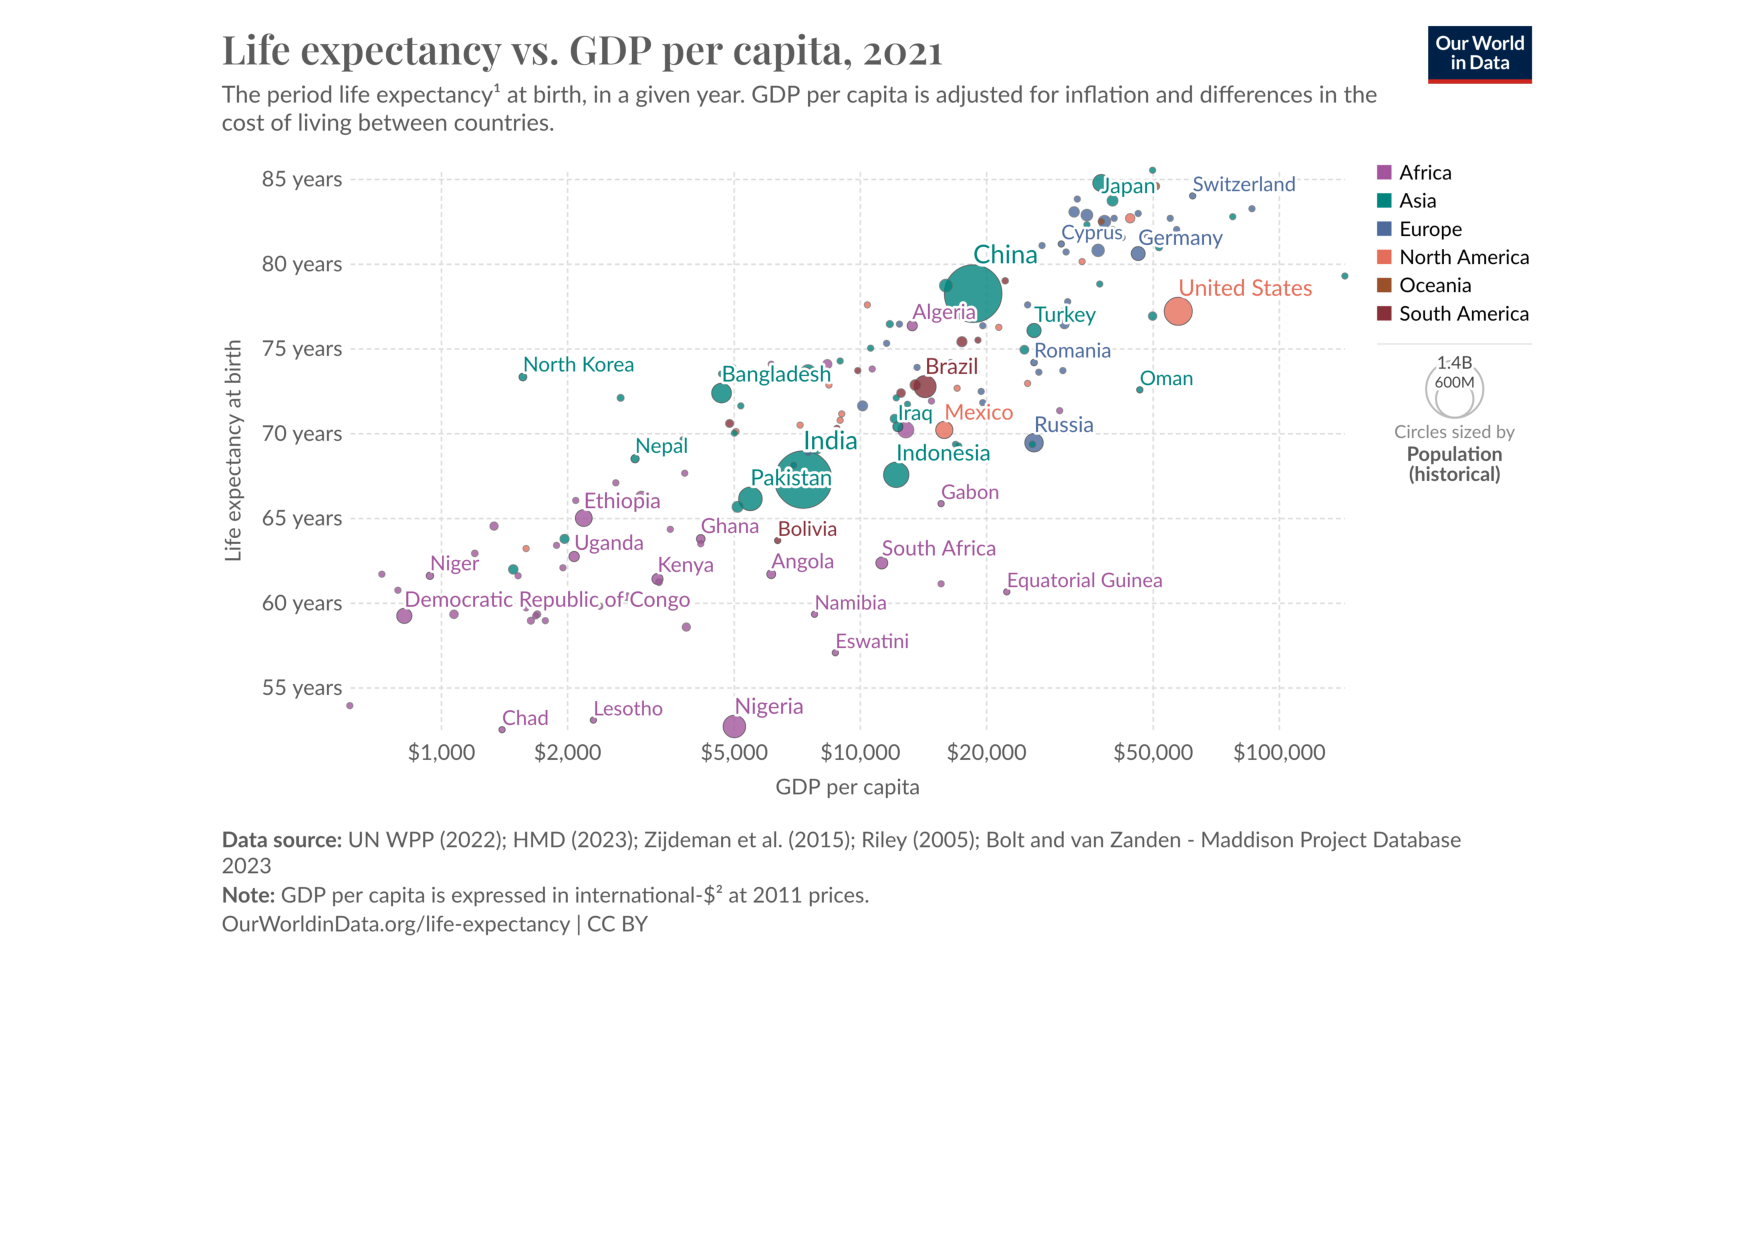
\includegraphics[width=\linewidth]{life-expectancy-vs-gdp-per-capita.pdf}
        \label{fig:enter-label}
    \end{figure}
\end{frame}

\begin{frame}{GDP and Child Mortality}
    \begin{figure}
        \centering
        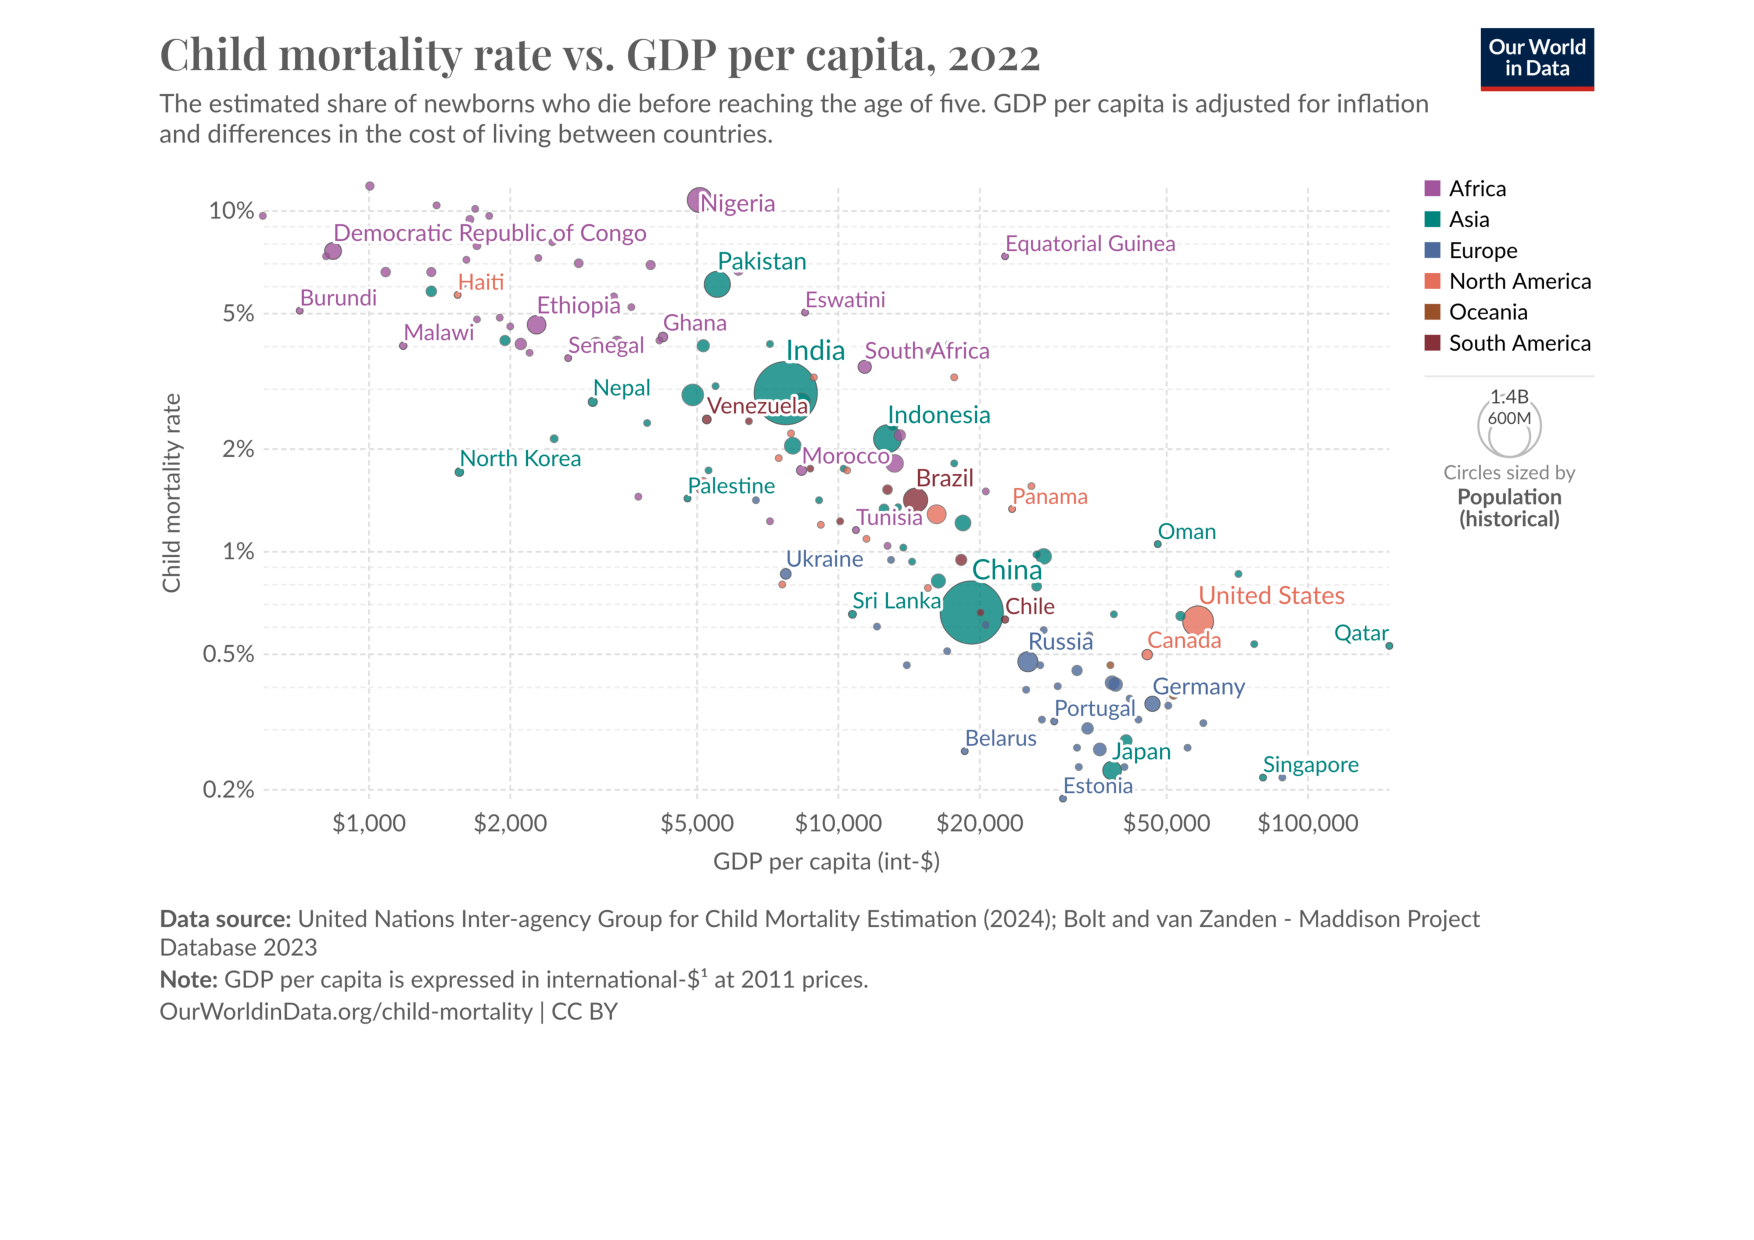
\includegraphics[width=1.08\linewidth]{child-mortality-gdp-per-capita.pdf}
        \label{fig:enter-label}
    \end{figure}
\end{frame}

\begin{frame}{Negative Impacts of Trade on Health}
\textbf{Channels}
\begin{itemize}
    \item Spread of infectious diseases % can happen at ports, through international business trips, much more interaction around the globe
    \item Dietary changes through a change in food items available % trade is introducing food from all around the world into local supermarkets but those choices aren't necessarily always the healthiest ones. They might be a cheap option because of hyperprocessed industrial processes, but that doesn't mean that they should be preferred
    \item Economic growth and associated environmental impact % last week I presented a paper that was concerned with Cap and Trade system in California
    \begin{itemize}
        \item pollution inequalities, global warming, plastic pollution that enters our food system 
    \end{itemize}
    \item Mental distress on workers in trade-exposed industries
    \begin{itemize}
        \item Drug abuse, depression and suicide rates 
    \end{itemize}
\end{itemize}
\end{frame}

\begin{frame}{GDP and CO2 Emissions}
     \begin{figure}
        \centering
        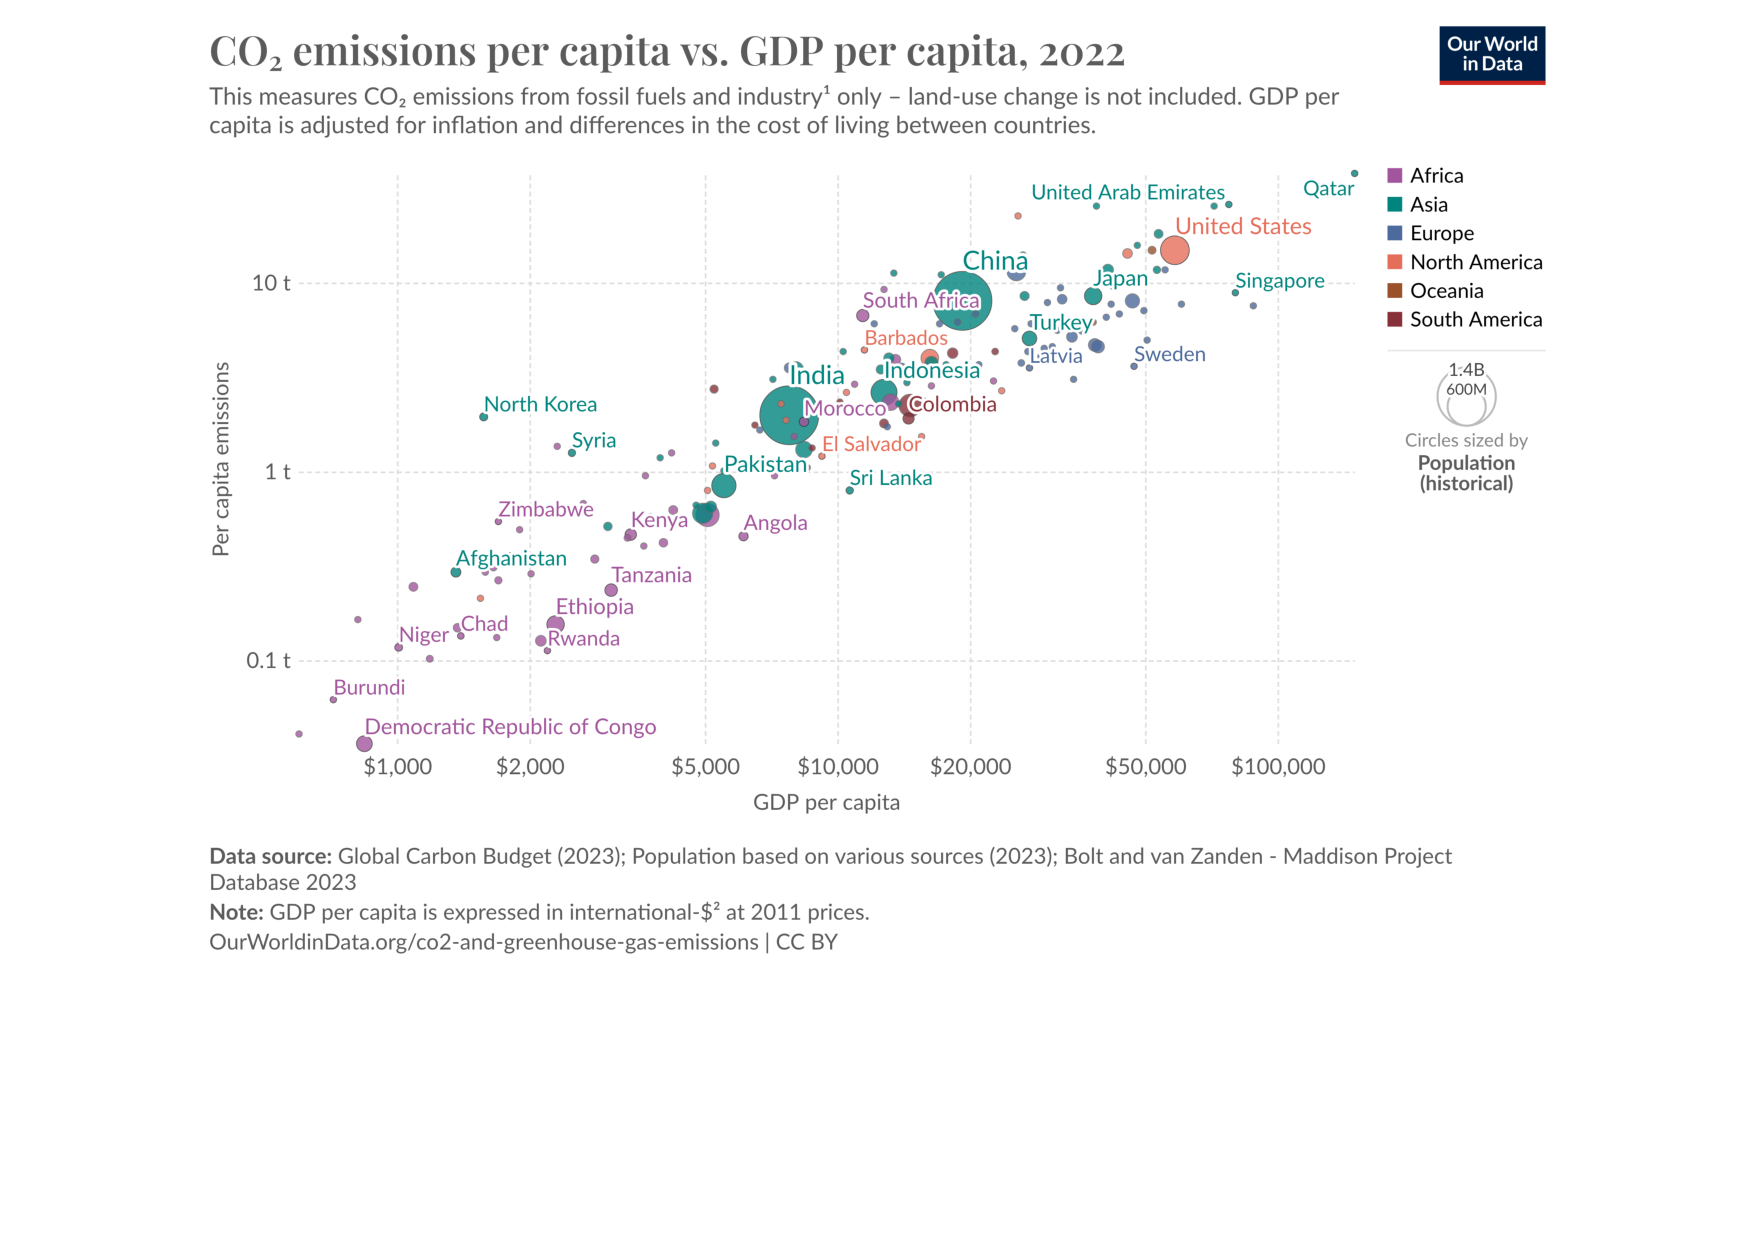
\includegraphics[width=\linewidth]{co2-emissions-vs-gdp.pdf}
        \label{fig:enter-label}
    \end{figure}
\end{frame} 

\begin{frame}{GDP and Death Rate from Outdoor Air Pollution}
     \begin{figure}
        \centering
        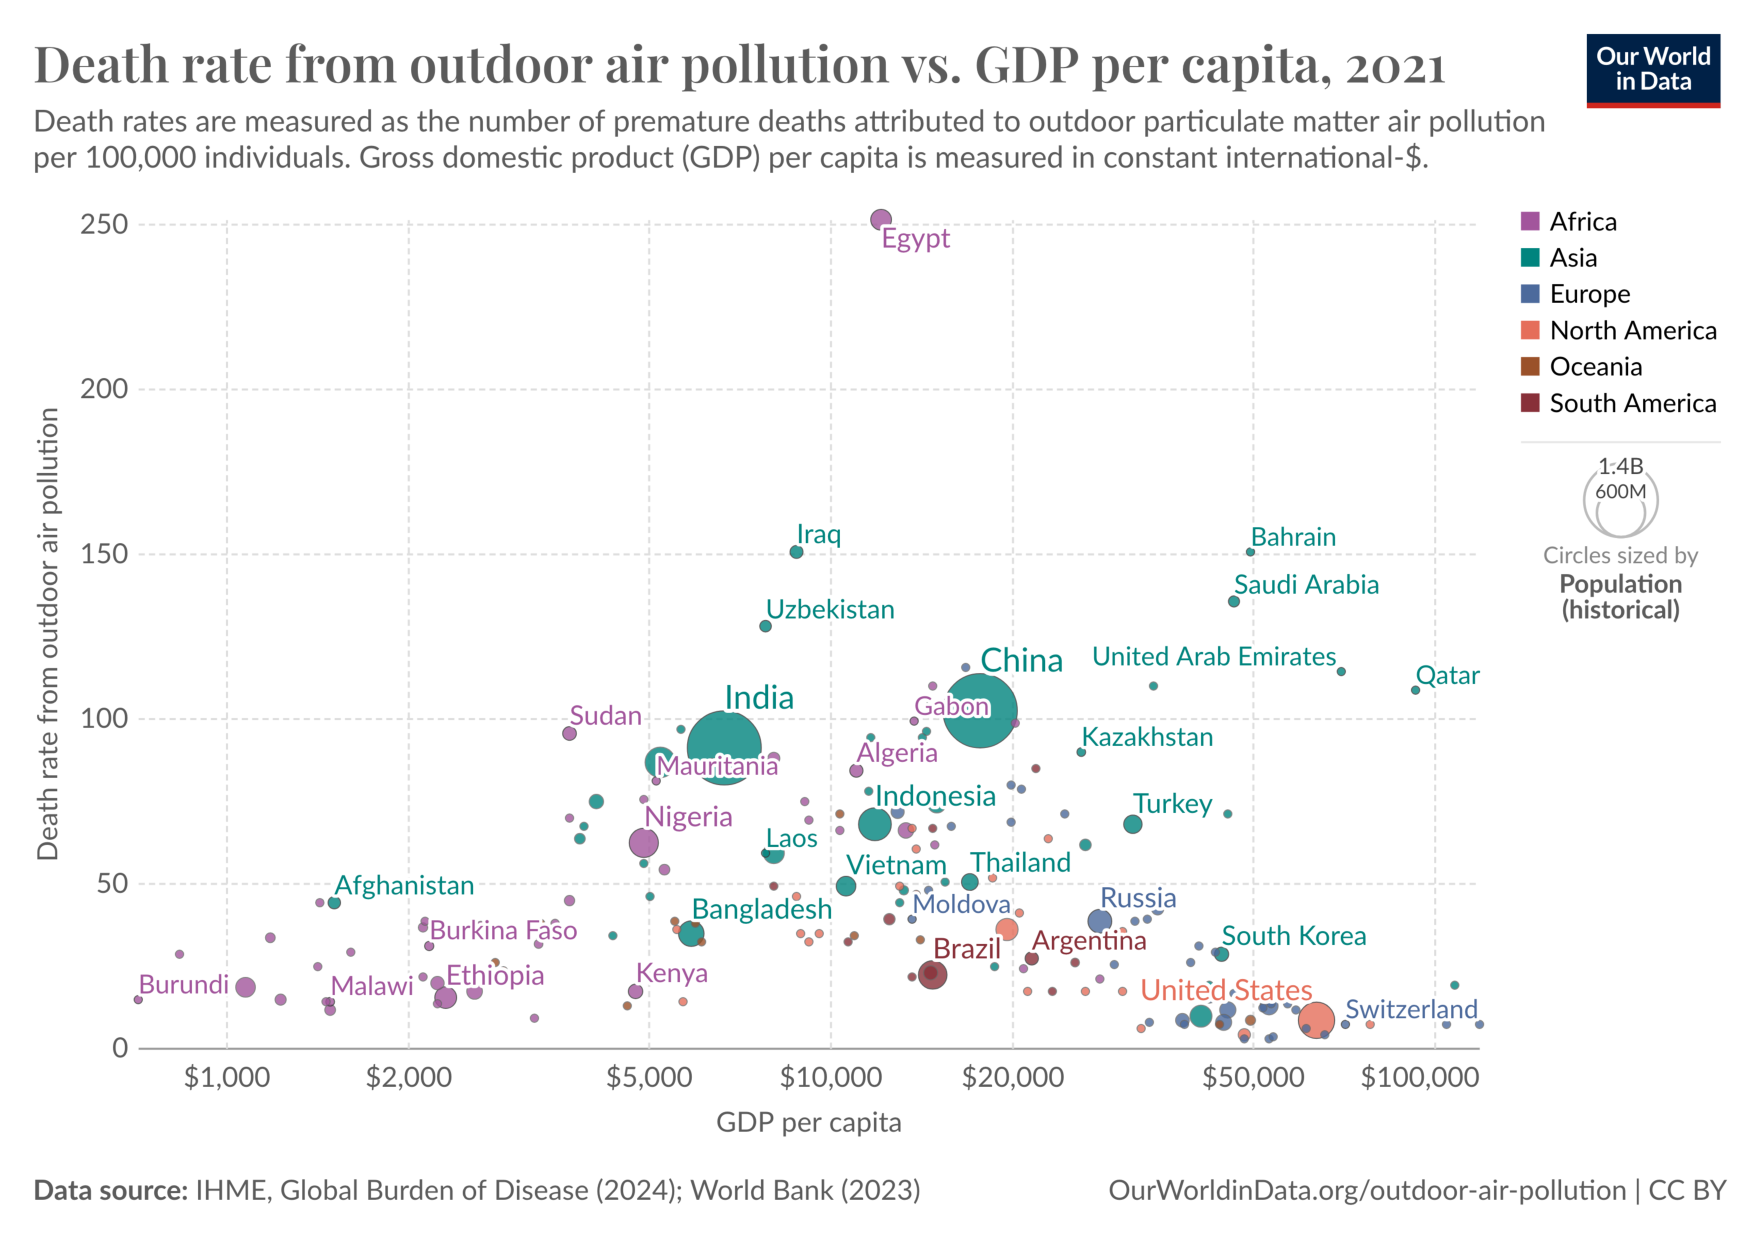
\includegraphics[width=0.9\linewidth]{outdoor-pollution-rate-vs-gdp.pdf}
        \label{fig:enter-label}
    \end{figure}
\end{frame}
% if you want to see it, you can see an enviornmental kuznets curve. It does seem to exist for local pollution like freshwater pollution for example.

\begin{frame}{Case Studies - Examples of Trade's Impact on Health}
    \begin{itemize}
        \item \textbf{Canada-U.S. Free Trade Agreement and Obesity}:
            \begin{itemize}
                \item Research links the agreement to increased calorie availability and higher obesity rates in Canada (\cite{barlow2018impact}).
                \item U.S. food exports led to changes in Canadian dietary patterns.
            \end{itemize}
        \item \textbf{The Spread of Smallpox along the Silk Roads}:
            \begin{itemize}
                \item Many viruses were transmitted via movement on the Silk Roads.
                \item The roads were not only transmitting diseases, but also medical knowledge and distributed some of the first versions of smallpox vaccination. 
            \end{itemize}
        \item \textbf{Pollution-related deaths in China from foreign Demand}:
            \begin{itemize}
                \item Increased trade led to higher and more localised pollution from certain industries, impacting respiratory health and causing deaths (\cite{china_air_pollution})
            \end{itemize}
    \end{itemize}
\end{frame}

\section{Health Effects on Trade}
\begin{frame}{Channels}
    \begin{itemize}
        \item Health crises, especially pandemics, can significantly disrupt global trade and supply chains through closed production, import bans and travel restrictions.
        \item Such events impact the labor force but also consumer demand.
        \item Example: COVID-19 showcased the global trade implications of a major health crisis with associated port closures and limited transportation options.
    \end{itemize}
\end{frame}

\begin{frame}{Economic Losses and Reduced Productivity}
    \begin{itemize}
        \item \textbf{Labor Shortages}: High infection rates reduce the workforce.
        \item \textbf{Decrease in Production Capacity}: Factories and businesses close due to quarantine restrictions, reducing trade volume.
        \begin{itemize}
            \item Production is additionally limited through dependency on intermediate goods from international supply chains.
        \end{itemize}
        \item Reduced production leads to a reduced income, which in itself decreases demand and production.
        \item Example: COVID-19 led to an economic shock as productivity declined globally.
    \end{itemize}
\end{frame}

\begin{frame}{Policy Responses and Trade Restrictions}
    \begin{itemize}
        \item \textbf{Health and Safety Regulations}: Increased restrictions on the import of goods, especially food and medical supplies.
        \item \textbf{Export Controls}: Many countries restrict exports of essential goods during pandemics.
        %\item Impact on Trade Relations: Strained relationships between trade partners due to export bans and restrictions can persist even after the immediate crisis is over.
    \end{itemize}
\end{frame}

\begin{frame}{Long-Term Effects and Recovery}
\textbf{Examplary Responses to Global Health Crises}
    \begin{itemize}
        \item \textbf{Reshaping of Supply Chains}: Many countries seek to diversify suppliers to reduce dependency.
        \item \textbf{Icreased Autonomy}: Another way of reducing international dependency is to invest more in the domestic production of vaccines, medical supply, essential food items, etc.
         \item \textbf{Increased Demand for Health-Related Trade}: Greater focus on importing medical supplies and pharmaceuticals (stockpiling).
    \end{itemize}
\end{frame}


\section{Empirical Papers}
\subsection{Globalization and Mental Distress}
\begin{frame}{Title Slide}
\begin{center}
    \begin{LARGE}
        Globalization and Mental Distress \\
    \end{LARGE}
    \begin{Large}
        by Italo Colantone, Rosario Crino, and Laura Ogliari \\
    \end{Large}
    In: Journal of International Economics (2019)
\end{center}
\end{frame}

\begin{frame}{Research Motivation}
    \begin{itemize}
        % \item Rising anti-globalization sentiments that can't exclusively be explained by economic factors.
        \item Existing evidence showing potential links between economic structural changes and drug abuse and suicide rates. % economists focussing on non-monetary impacts of increased international trade
        \item Motivation to provide individual-level (micro) insights into trade-related mental health impacts.
    \end{itemize}
    \begin{tcolorbox}
        \textbf{Research Question:} What is the causal impact of increased import competition on the mental distress of workers employed in trade-exposed industries?
    \end{tcolorbox}
\end{frame}

\begin{frame}{Literature Review}
    \begin{itemize}
        \item Trade exposed localities exhibit higher mortality rates due to suicides and drug overdoses (\cite{adda2017health}, \cite{pierce2020trade})
        \item Further literature discusses a number of new non-monetary effects of import competition: increases in local area crime, household debt, job-related injuries, as well as fertility and marriage rates.
        \item However, there is limited evidence on import competition’s effects on individual mental health.
    \end{itemize}
\end{frame}

\begin{frame}{Hypothesis}
    \begin{itemize}
        \item \textbf{Hypothesis}: Increased import competition leads to higher mental distress.
        \item \textbf{Channels}: \pause 
        \begin{enumerate}
            \item Increased probability of job displacement.
            \item Reduced wage growth for non-displaced workers.
            \item Lower job satisfaction.
            \item Gloomier expectations about the future.
        \end{enumerate} 
        %\item Focus: Analyzing individual mental health survey responses over time.
    \end{itemize}
\end{frame}

\begin{frame}{Data}
    \textbf{British Household Panel Survey}
    \begin{itemize}
        \item Longitudinal representative dataset tracking individuals in the UK from 1991 to 2009.
        \item Provides detailed mental health and employment data for all surveyed individuals.
        \item Allows to check for spillover effects within households.
        \end{itemize}
        \textbf{Import Data}
        \begin{itemize}
        \item Data on import competition by industry over 1995-2007. Import competition is thereby measured as the growth in imports in that specific industry.
    \end{itemize}
\end{frame}

\begin{frame}{Key Variables}
    \begin{itemize}
        \item \textbf{Mental Health Measure}: GHQ-12, a standardized mental distress indicator.
        \item \textbf{Import Competition}: Calculated from import growth in each industry.
        \item Control variables include demographics, household factors, and job characteristics.
    \end{itemize}
\end{frame}

\begin{frame}{Methodology}
    \begin{itemize}
        \item Instrumental variable (IV) approach to address endogeneity concerns. % at this point, draw the graph on instrumental variable approach
        \begin{itemize} \pause
            \item Instead of accessing the effect of import growth per industry, the authors proxy the true growth in imports by a baseline share of exporting countries interacted with their export in that industry per year $\rightarrow$ shift-share instrument.
            \item The instrument is meant to isolate the variation in UK imports that is due to changes in supply conditions in foreign countries, rather than to domestic industry-specific shocks in the UK. % if the domestic industry in textile is doing badly because they are not as technologically advanced as some other countries and as a result, the UK imports more textile from abroad, the mental distress in this UK industry might not be the outcome of the increase in trade, but rather has something to do with the domestic industry
        \end{itemize}
        \item Main identification strategy: Compare GHQ-12 scores across similar individuals in industries hit by different degrees of trade shocks.
    \end{itemize}
\end{frame}

\begin{frame}{Main Results}
    \begin{itemize}
        \item Increased import competition significantly increases mental distress of workers.
        \item A one standard deviation increase in import competition raises GHQ-12 by 1.15 percentage points.
    \end{itemize}
\end{frame}

\begin{frame}{Results - Heterogeneity Analysis}
    \begin{itemize}
        \item Younger workers, those with families, and blue-collar workers show greater distress.
        \item Temporary contract and lower-wage workers are more vulnerable to mental health impacts.
        \item Impact is larger among workers with less job security and financial stability.
    \end{itemize}
    Overall, the effect is largest for those workers with the least economic stability.
\end{frame}

\begin{frame}{Results - Intra-Household Effects}
     \textbf{Trade exposure of one family member affects the mental health of other family members.}
    \begin{itemize}
        \item Women’s mental distress increases due to partners' trade exposure.
        \item Negative impacts on children’s self-esteem and life satisfaction.
    \end{itemize}
\end{frame}

\begin{frame}{Discussion}
    \begin{itemize}
        \item Findings indicate that import competition has significant non-monetary costs for affected industries and the people employed in those.
        \item Trade exposure decreases the mental health level of female spouses but not male ones. \textbf{Why?} \pause
        \item External validity is unlikely to hold. % the UK is a highly industrialised country, it has workers rights a healthcare system, social security etc. the effect of increased international competition on mental distress is unlikely to be representative for all workers
        \begin{itemize}
            \item The size of the effect is likely determined by the size of the welfare state and social security system.
        \end{itemize}
    \end{itemize}
\end{frame}

\begin{frame}{Conclusion}
    \begin{itemize}
        \item Import competition significantly increases mental distress among UK workers.
        \item \textcite{globalization_and_mental_distress} deliver the first comprehensive evidence on the heterogeneous effects across workers within exposed industries as well as family spillover effects.
        \item Heightened trade competition can amplify existing inequalities even within the same industry.
        \item Trade exposure systematically hits individuals hardest, whose characteristics make them structurally less resilient and more vulnerable to shocks.
    \end{itemize}
\end{frame}


\subsection{The Impact of U.S. Free Trade Agreements on Calorie Availability and Obesity}

\begin{frame}{Title Slide}
\begin{center}
    \begin{LARGE}
        The Impact of U.S. Free Trade Agreements on Calorie Availability and Obesity: \\ A Natural Experiment in Canada \\
    \end{LARGE}
    \begin{Large}
        by Pepita Barlow, Martin McKee, and David Stuckler \\
    \end{Large}
    In: American journal of preventive medicine (2018)
\end{center}
\end{frame}

\begin{frame}{Research Question and Motivation}
\textbf{Motivation and Background:}
    \begin{itemize}
    \item Large amounts of scientific evidence positively correlate the Western diet to acne, obesity, diabetes, heart disease and cancer, the so-called “diseases of civilization” (\cite{civilization_disease}). 
    %\item Globalization has facilitated the spread of such diets. % increased availability of highly processed food and beverages. Furthermore, we have higher competition for remaining goods in the supermarket, which is decreasing prices, domestic production in the food sector is increasing as well and this could all lead to an overconsumption. Greater marketing
    \item Free Trade Agreements (FTAs) reduce trade barriers (including the food sector). %  whether or not FTAs contribute to rising obesity depends, in part, on whether they increase peoples’ net caloric intake
    \item Previous studies lack causal inference. \textcite{barlow2018impact} use a natural experiment approach: the Canada–U.S. Free Trade Agreement (CUSFTA) of 1989. % the implementation was contingent on the Canadian election in 1988, which was a very close election and so the implementation was as if random
    \end{itemize}
    \begin{tcolorbox}
        \textbf{Research Question}: How did the Canada-U.S. Free Trade Agreement affect calorie availability in Canada?
    \end{tcolorbox}
\end{frame}

\begin{frame}{Data and Sample}
    \begin{itemize}
        \item Data from the UN Food and Agriculture Organization (FAO) on calorie availability (1978–2006). % this is a flow measure: what is produced and coming into the country per year? what is exported? what is used to feed to animals? the rest is for humans. How many humans do we have in the country? -> calorie availability
        \item Trade and investment data from U.S. Bureau of Economic Analysis and U.S. Department of Agriculture.
        \item Data on country-level covariates stems from the World Bank World Development Indicators
        \item Comparison countries: Denmark, the Netherlands, and New Zealand.
    \end{itemize}
\end{frame}

\begin{frame}{Methodology}
    \begin{itemize}
        \item \textbf{Fixed-Effects Regression}: Compares calorie availability before and after CUSFTA.
        $$Y_{it} = \alpha_0 +\gamma_i + \beta D_{it} + \theta X_{it} + \epsilon_{it}$$
        \item \textbf{Synthetic Control Method}: The authors create their own counterfactual(s): a synthetic Canada created from control countries.
    \end{itemize}
\end{frame}

\begin{frame}{Calorie Availability - Fixed-Effects Regression}
    \begin{figure}
        \centering
        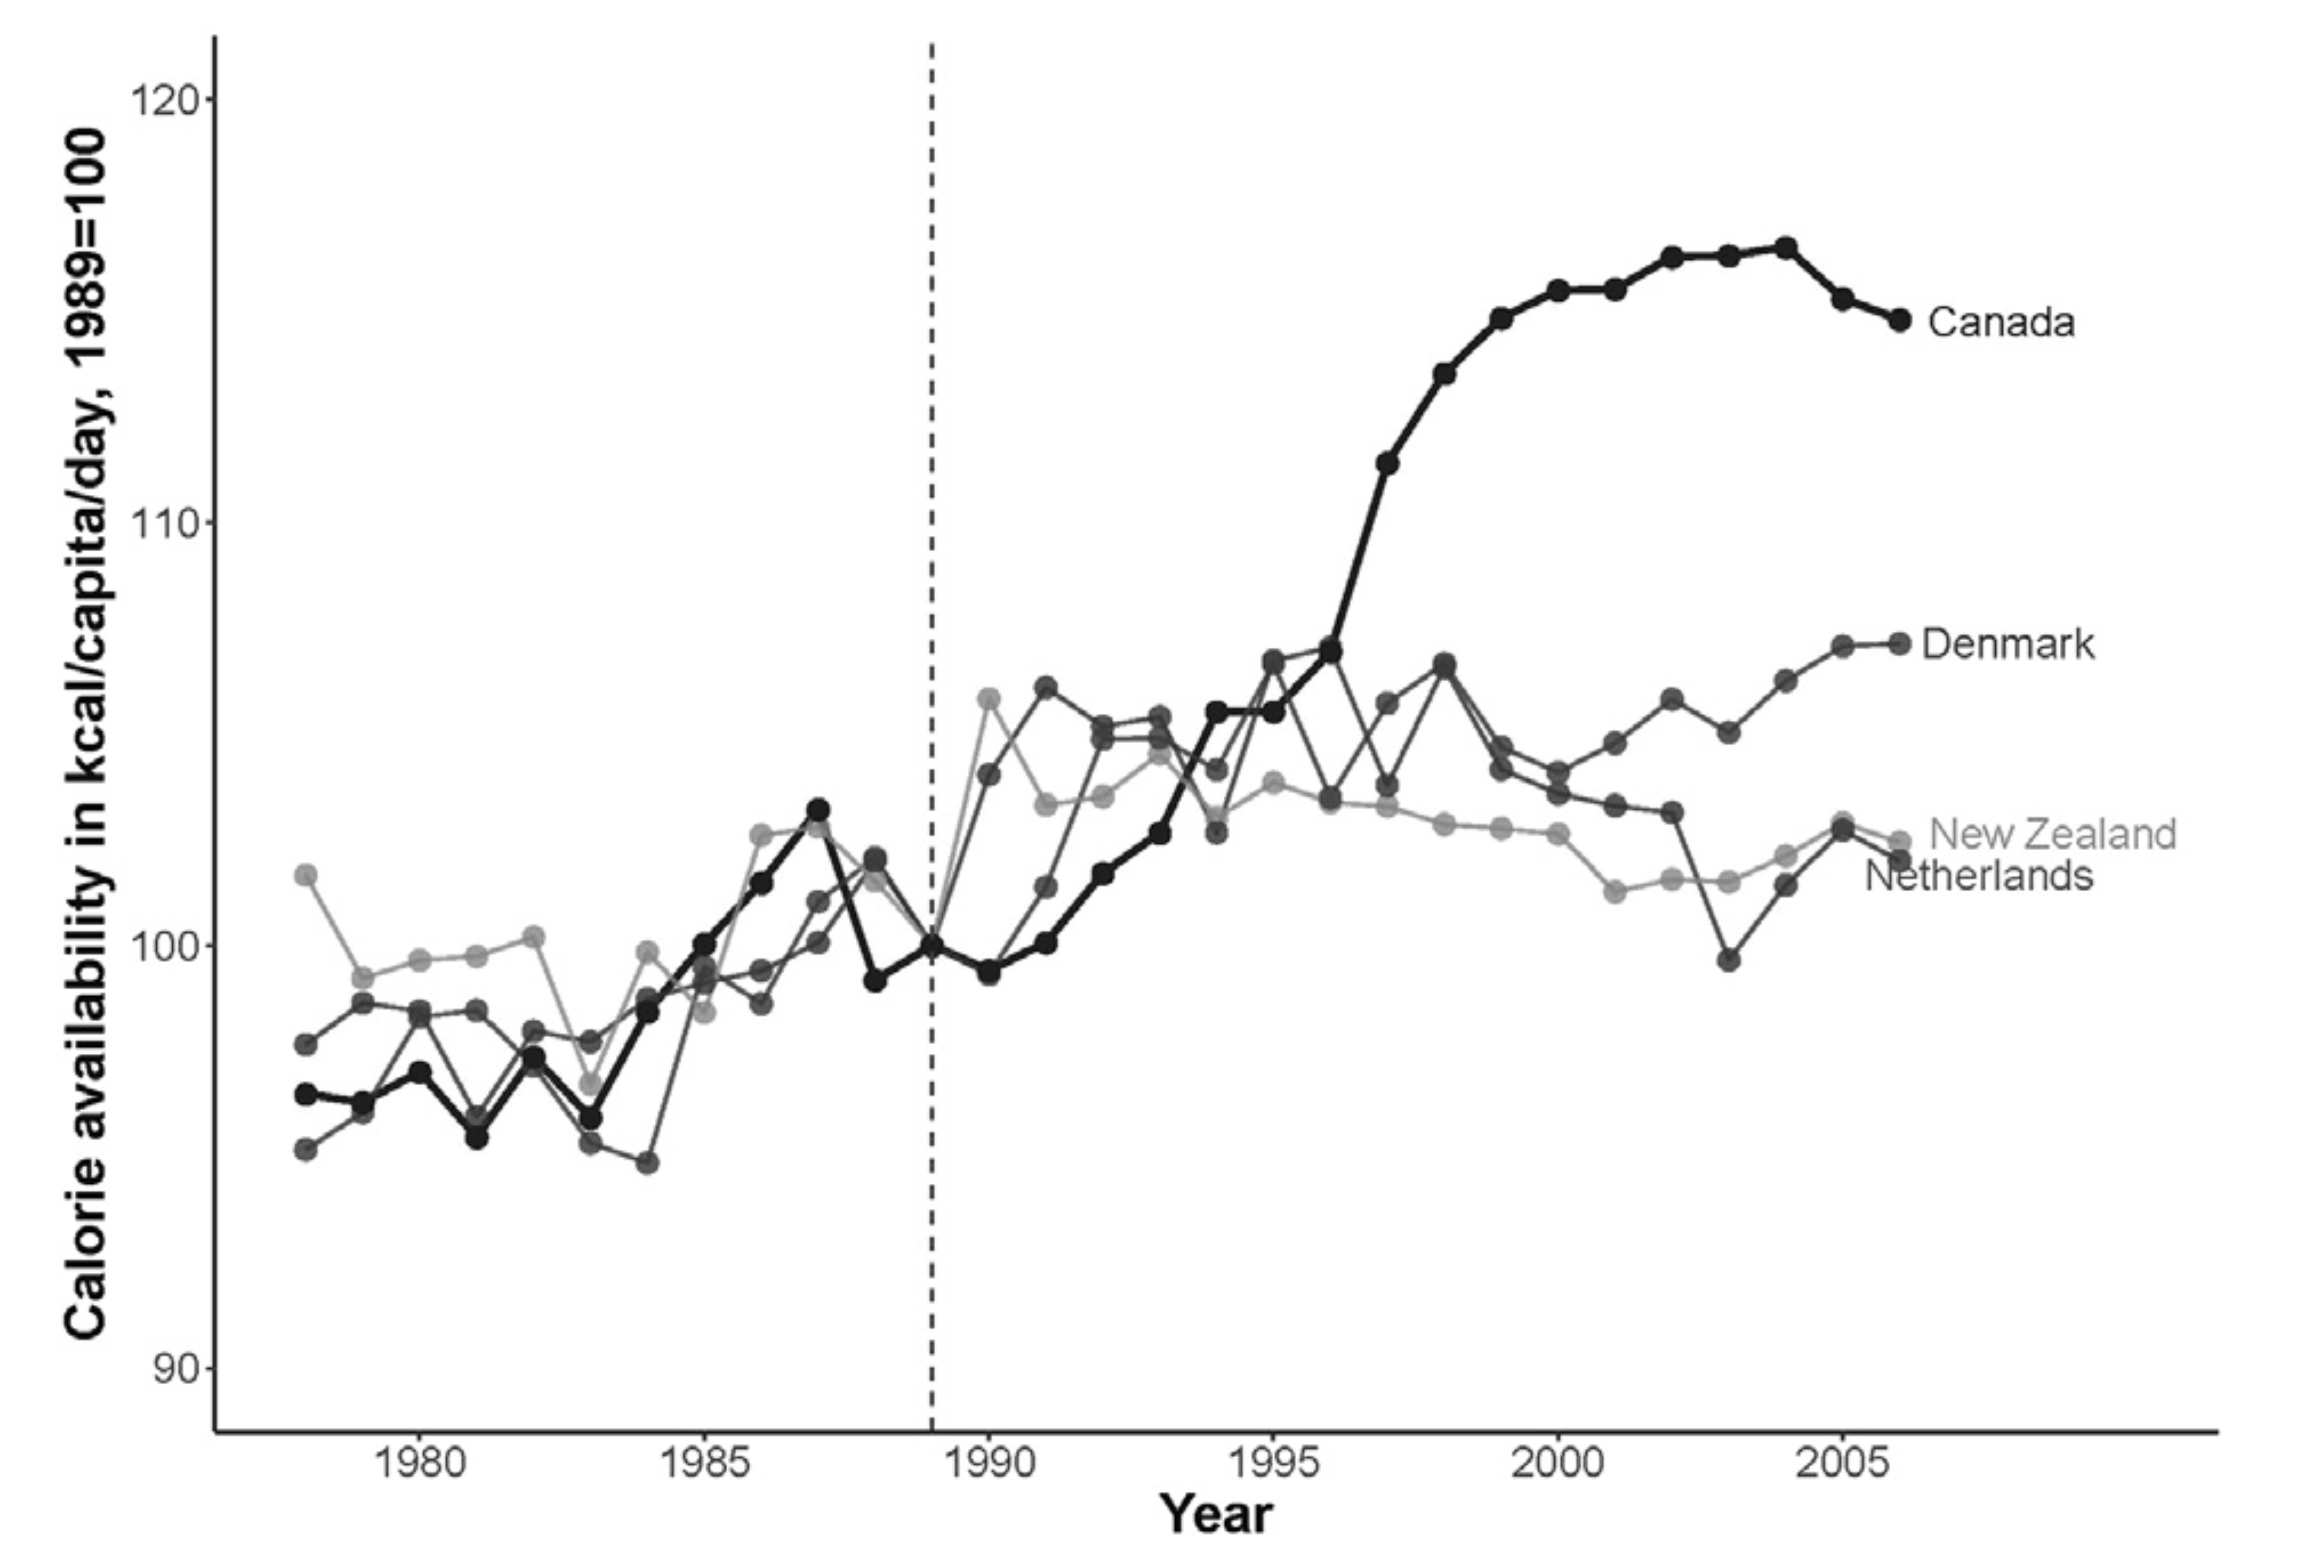
\includegraphics[width=0.8\linewidth]{Bildschirmfoto 2024-11-07 um 10.22.36.png}
        \caption{Source: \textcite{barlow2018impact}}
        \label{fig:enter-label}
    \end{figure}
\end{frame}

\begin{frame}{Calorie Availability - Synthetic Control}
    \begin{figure}
        \centering
        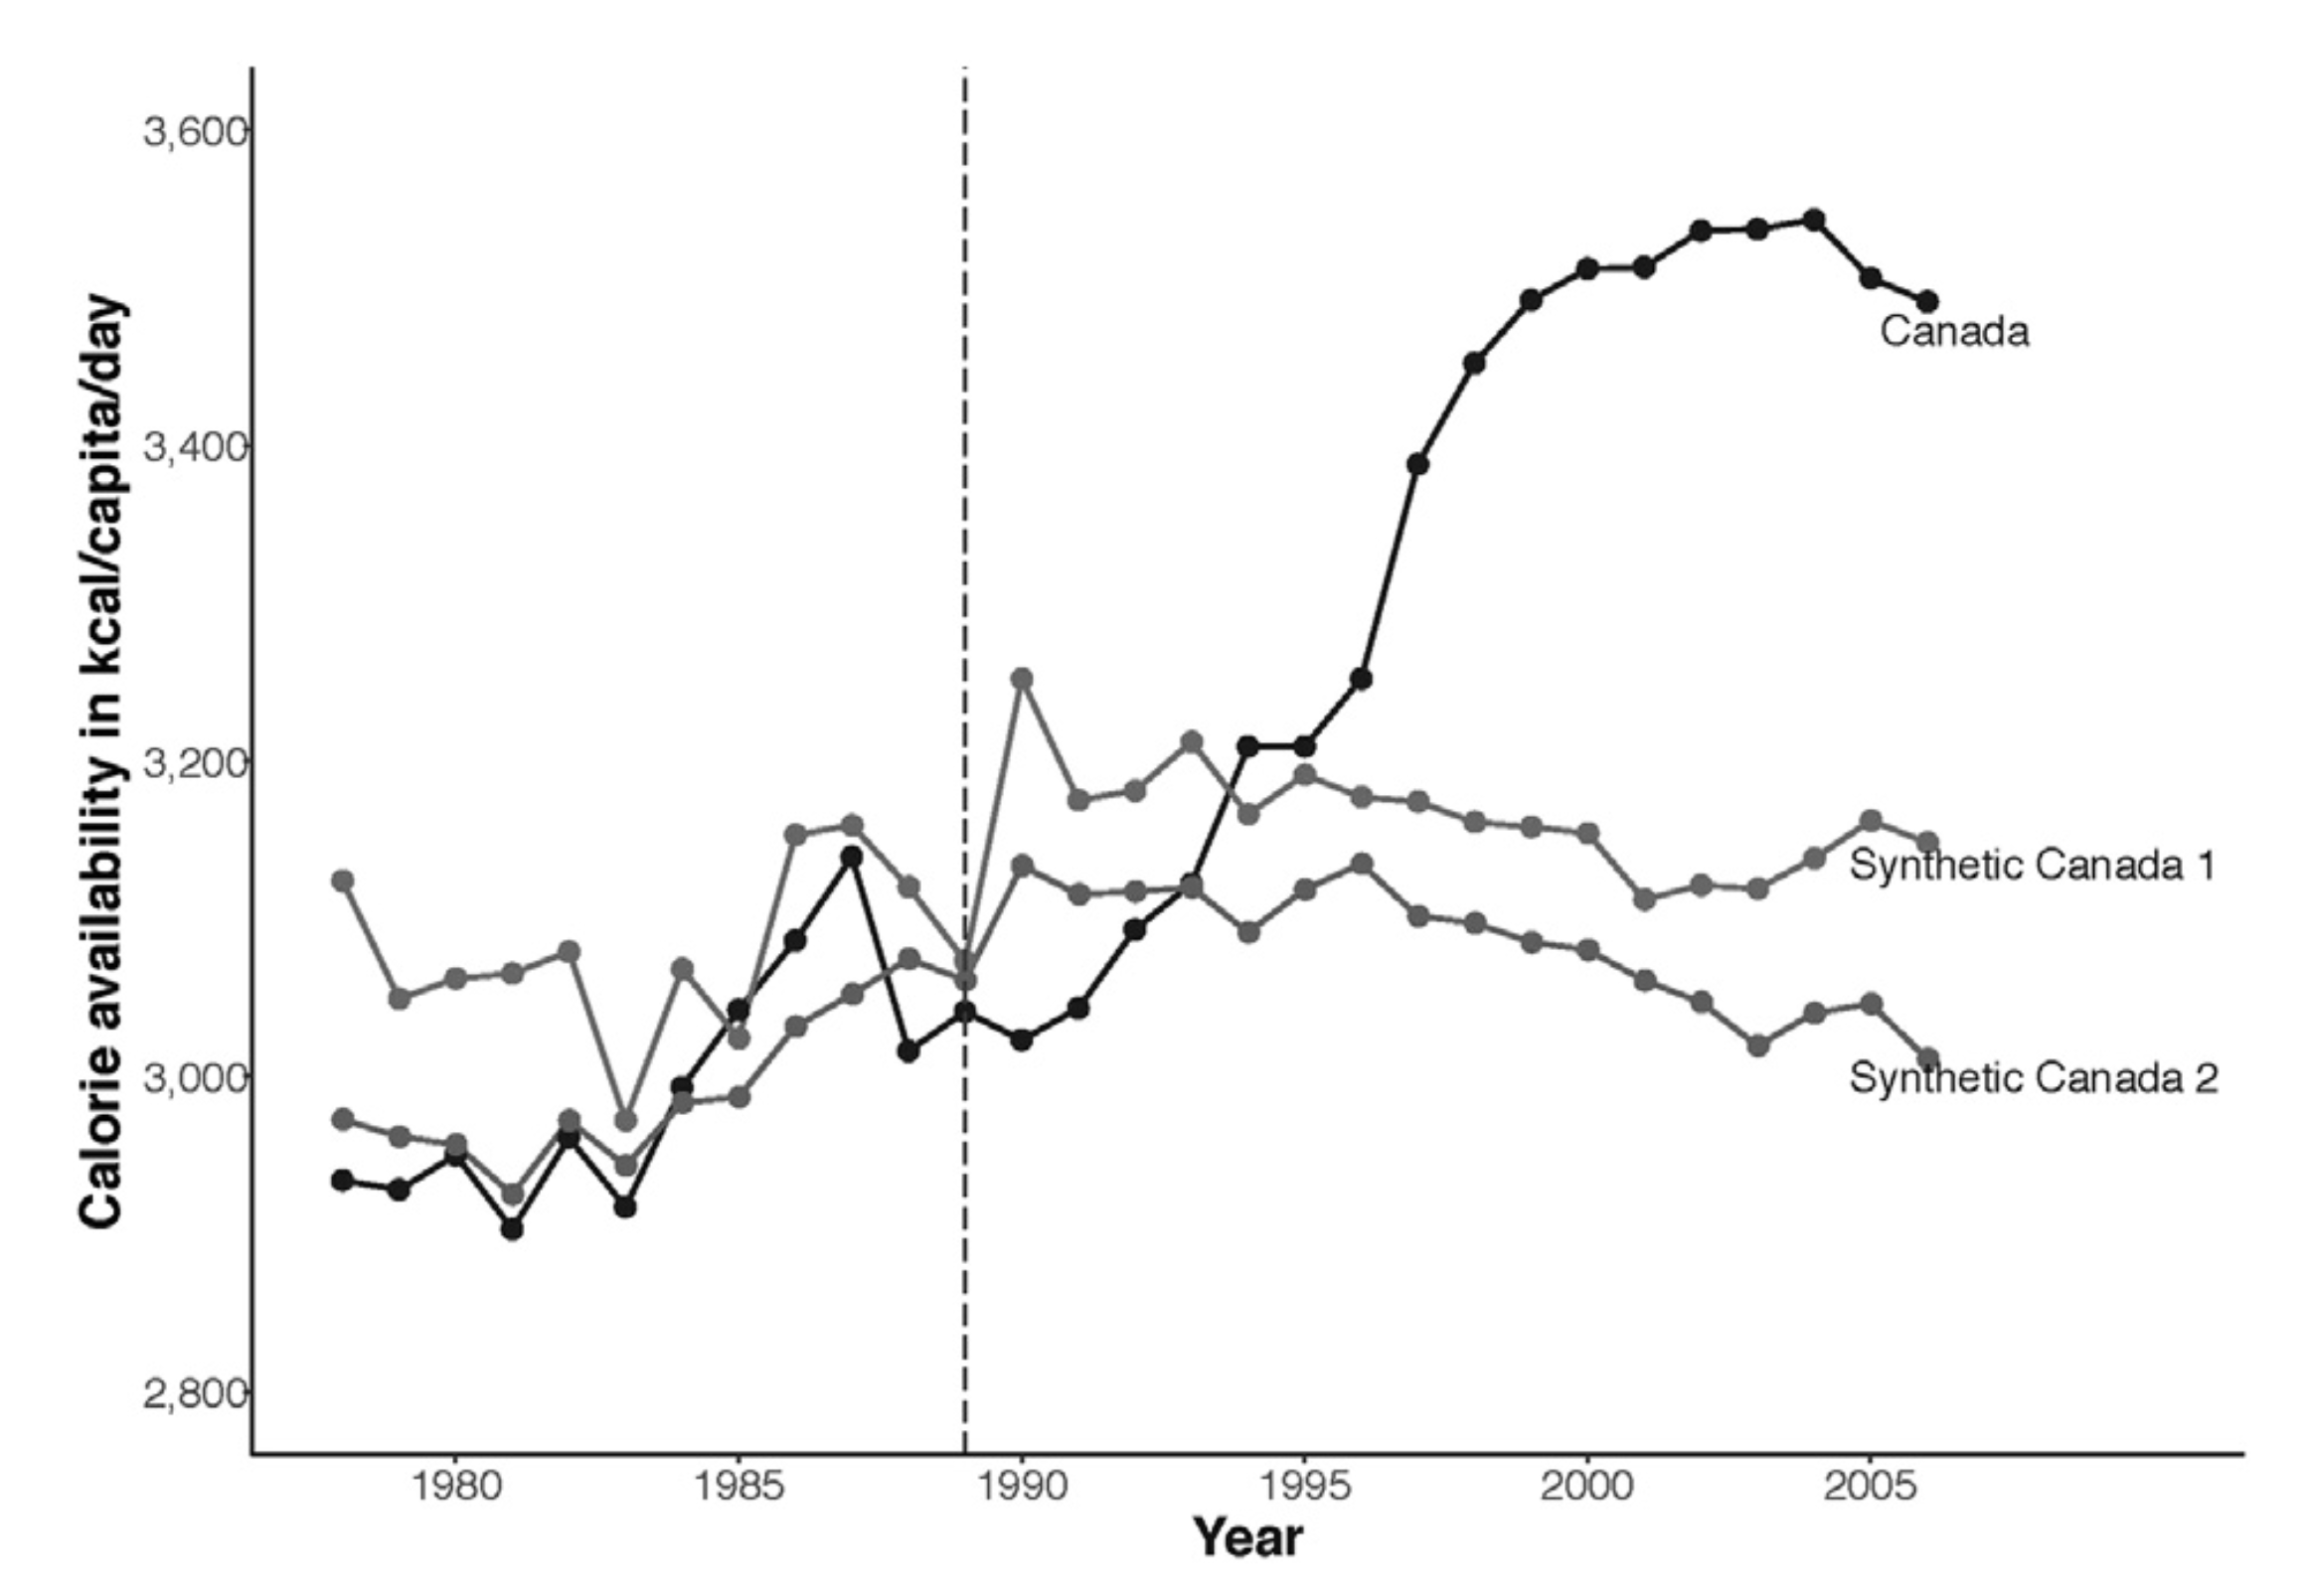
\includegraphics[width=0.8\linewidth]{Bildschirmfoto 2024-11-07 um 10.36.08.png}
        \caption{Source: \textcite{barlow2018impact}}
        \label{fig:enter-label}
    \end{figure}
\end{frame}

\begin{frame}{Main Results}
    \begin{itemize}
      \item The trade agreement led to a rise in U.S. trade and investment in Canada’s food sector.
        \item \textcite{barlow2018impact} find that calorie availability increased by $\approx$170 kcal per person per day after CUSFTA. This equivalates to one cup of orange juice or half of a standard milk chocolate bar. 
        \item Effect consistent across different model specifications proposed by the researchers.
    \end{itemize}
\end{frame}

\begin{frame}{Discussion and Limitations}
    \begin{itemize}
        \item \textbf{Discussion}: CUSFTA demonstrates how trade agreements can influence national diets and health outcomes, thereby highlighting those consideration in trade policy.
        \item \textbf{Limitations}:
            \begin{itemize}
                \item Calorie availability as a proxy for intake is likely overestimating actual consumption.
                \item The study does not directly measure obesity or weight data.
                \item Had calorie supply in Canada been insufficient before CUSFTA, the FTA would not have increased obesity but increased health.
                %\item The controls used could have biased the results (GDPPC and urbanization).
            \end{itemize}
    \end{itemize}
\end{frame}

\begin{frame}{Conclusion}
    \begin{itemize}
        \item CUSFTA was associated with a substantial rise in calorie availability in Canada.
        \item Findings suggest FTAs can impact health by influencing dietary intake.
        \item Future research should explore trade’s effects on other dietary and health outcomes and actual obesity rates by working with weight data.
    \end{itemize}
\end{frame}



\begin{frame}[allowframebreaks]{References}
    \printbibliography
\end{frame}


\end{document}

